\chapter{Modelação da Base de Dados}

\paragraph{}

Resumidamente a base de dados está representada da seguinte forma:

\begin{list}{\textbf{-}}{\textbf{TABELAS}}
\item \textbf{curso} - Representa os cursos leccionados
\item \textbf{ano\_lectivo} - Representa um ano lectivo
\item \textbf{utilizador} - todos os utilizadores ficam registados nesta tabela
\item \textbf{curso\_ano} - Representa um curso leccionado num determinado ano, nesta tabela fica representado o coordenador do curso nesse ano associando o id do respectivo user na tabela utilizador
\item \textbf{semestre} - Representa um semestre de um determinado ano lectivo
\item \textbf{disciplina} - Representa uma disciplina
\item \textbf{disciplina\_semestre} - Faz referencia a uma disciplina leccionada num determinado semestre
\item \textbf{Docente} - Representa um ou mais utilizadores designados como docentes de uma determinada disciplina
\item \textbf{aluno} - Representa uma matrícula de um utilizador como aluno num determinado curso
\item \textbf{matricula\_disciplina} - Representa a matricula numa disciplina de um determinado aluno
\item \textbf{avaliacao} - Representa uma avaliacao marcada para uma disciplina leccionada num determinado semestre
\item \textbf{avaliacao\_datas\_alt} - Nesta tabela ficam registadas as datas alternati vas escolhidas pelo docente para que o coordenador possa ter a possibilidade de trocar caso aconteça um peso demasiado excessivo nas avaliações para os alunos.
\item \textbf{avaliacao\_aluno} - Representa a inscrição de um aluno numa avaliação e é onde fica registada a sua nota
\end{list}

\begin{list}{\textbf{-}}{\textbf{STORED PROCEDURES}}
\item \textbf{get\_coordinator\_evaluations( user\_num, num\_discipline )} - Obter lista de avaliações com o perfil de coordenador de um determinado utilizador
\item \textbf{get\_teacher\_evaluations( user\_num, num\_discipline )} - Obter lista de avaliações com o perfil de docente de um determinado utilizador
\item \textbf{get\_student\_evaluations( user\_num, num\_discipline )} - Obter lista de avaliações com o perfil de aluno de um determinado utilizador
\item \textbf{get\_cursos\_user( user\_num )} - Obter lista de cursos a que utilizador esteja associado
\item \textbf{get\_coordinator\_disciplines( user\_num, num\_course )} - Obter lista de disciplinas com o perfil de coordenador de um determinado utilizador
\item \textbf{get\_teacher\_disciplines( user\_num, num\_course )} - Obter lista de disciplinas com o perfil de docente de um determinado utilizador
\item \textbf{get\_student\_disciplines( user\_num, num\_course )} - Obter lista de disciplinas com o perfil de aluno de um determinado utilizador
\item \textbf{add\_evaluation( user\_num, discipline\_id, date, weight, classroom, type, observations )} - Adicionar uma avaliação a uma determinada disciplina
\end{list}

\begin{figure}[!htbp]
\centering
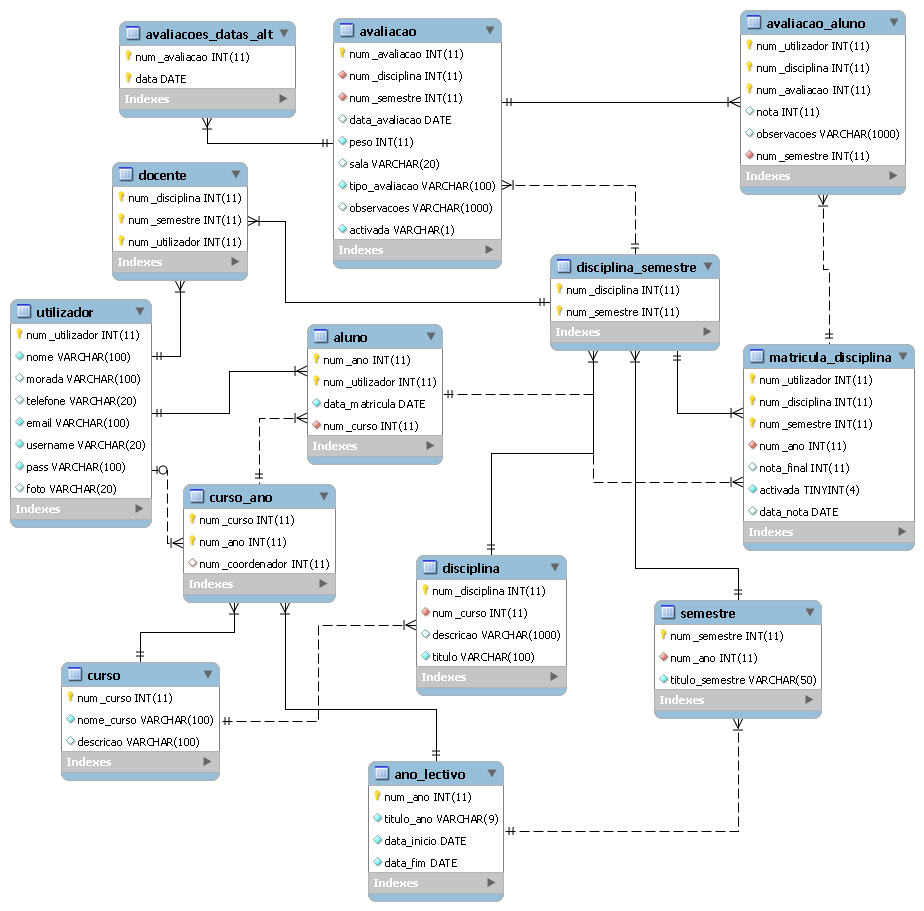
\includegraphics{imagens/base_de_dados.png}
\caption{Base de Dados: Modelo Físico}
\label{fig:modelo_fisico}
\end{figure}

